
\documentclass[a4paper,12pt]{article}
\usepackage[top=1.5cm,bottom=1.5cm,left=1.5cm,right=1.5cm]{geometry}
\usepackage[T1]{fontenc}
\usepackage[utf8]{inputenc}
\usepackage{newunicodechar}
\usepackage{lmodern}
\usepackage{textgreek}
\usepackage{amsmath}
\usepackage{mathtools}
\usepackage{graphicx}
\usepackage{pdflscape}
\usepackage{svg}

\usepackage{tabularx}
\usepackage{blindtext}
\usepackage{hyperref}
\usepackage{pgfgantt}
\usepackage{colortbl}
\usepackage{pdfpages}
\usepackage{setspace}
\usepackage{subcaption}
\usepackage{tikz}
\usepackage{chngcntr}
\usepackage{longtable}
\usepackage{xcolor,colortbl}
\usepackage{pdfpages}
%
\counterwithin{figure}{subsection}
\usepackage{multicol} 

\setcounter{tocdepth}{3}


\begin{document}
	
	\begin{titlepage}
		\newcommand{\HRule}{\rule{\linewidth}{0.5mm}}
		\begin{tikzpicture}[remember picture, overlay]
		\node [anchor=north east, inner sep=0pt]  at (current page.north east)
		{
\includegraphics[width=21cm]{../resources/graphics/ucl-banner-dl-port-outline.eps}};
		\end{tikzpicture}\\[3cm]
		\center
		
		\textsc{\Large University College London}\\[0.5cm]
		\textsc{\large Department of Electronic and Electrical Engineering}\\[0.5cm]
		
		\HRule \\[0.4cm]
		\setstretch{1.5}
		{ \huge \bfseries Project Progress Report No. 6}\\[0.4cm]
		\setstretch{1.0}
		\HRule \\[1.0cm]
		
		\Large \emph{Author:}\\
		Minduagas \textsc{Jarmolovičius}\\
		\href{mailto:zceemja@ucl.ac.uk}{zceemja@ucl.ac.uk}\\[0.5cm]
		
		\Large \emph{Supervisor:}\\
		Prof. Robert \textsc{Killey}\\
		\href{mailto:r.killey@ucl.ac.uk}{r.killey@ucl.ac.uk}
		\vfill
		
		{\large Match  25, 2020}\\[2cm]
		
	\end{titlepage}
	
\pagebreak
	
\section{Progress}
Tasks that been done since last progress report:

\subsection{Presentation and Final report}
Completed presentation \& started working on final project report.

\subsection{Power measurement}
Experiment been performed to measure power consumption of both processors at fixed frequency of 1MHz.

\begin{figure}[h!]
	\centering
	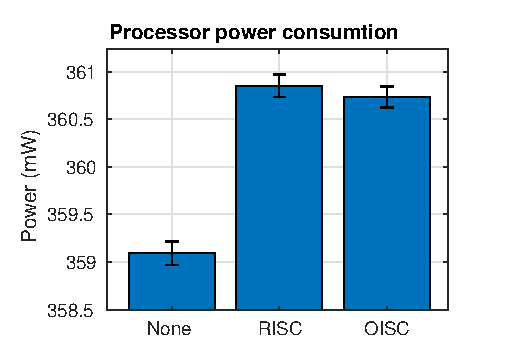
\includegraphics[]{../tests/power.eps}
	\caption{Measured power of processors when implemented on FPGA, running 16bit multiplication function in loop. None indicates auxiliary-only power.}
	\label{fig:power}
\end{figure}

\subsection{RISC programs}
Added RISC programs to calculate 16bit modulus and division.
Almost completed RISC Sieve of Atkins for 16bit.

\subsection{Function analysis}

\begin{figure}[b!]
	\centering
	\begin{subfigure}[b]{0.3\textwidth}
		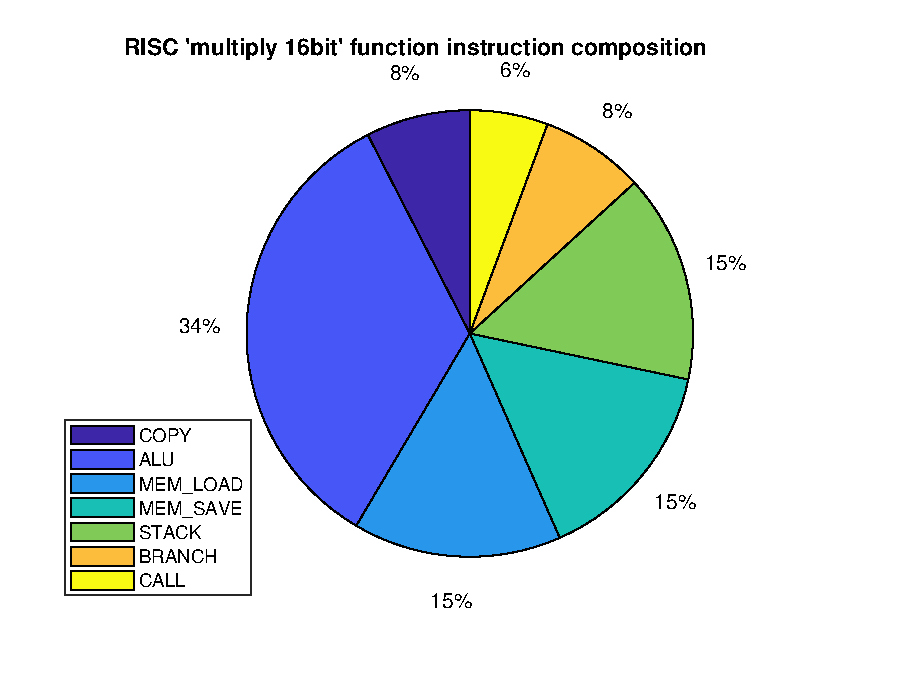
\includegraphics[width=1.3\textwidth]{../tests/risc_mul16_comp.eps}
		\caption{}
		\label{fig:t0}
	\end{subfigure}
	~
	\begin{subfigure}[b]{0.3\textwidth}
		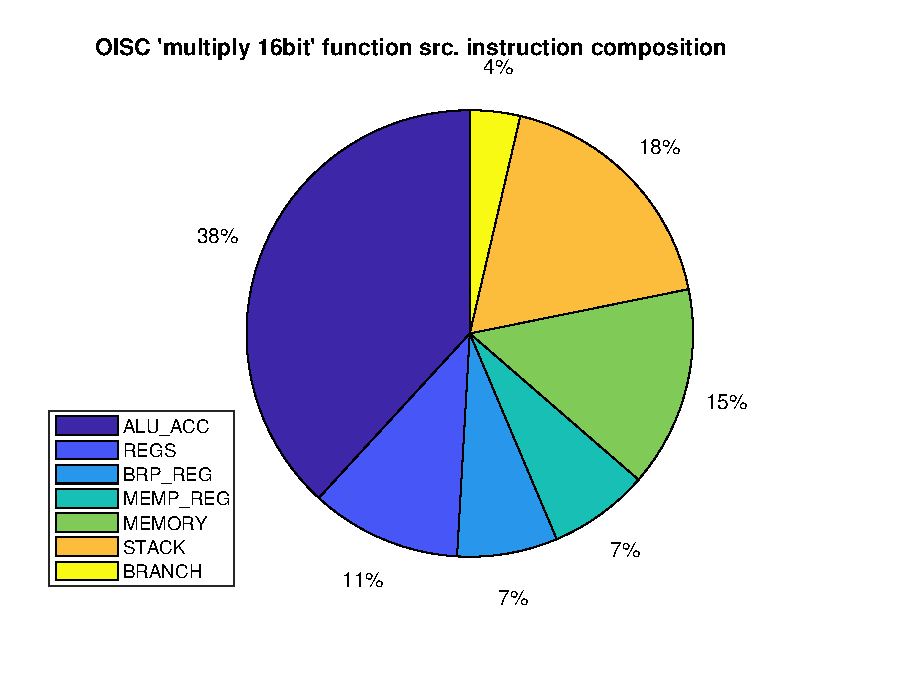
\includegraphics[width=1.3\textwidth]{../tests/oisc_mul16_src_comp.eps}
		\caption{}
		\label{fig:t1}
	\end{subfigure}
	~
	\begin{subfigure}[b]{0.3\textwidth}
		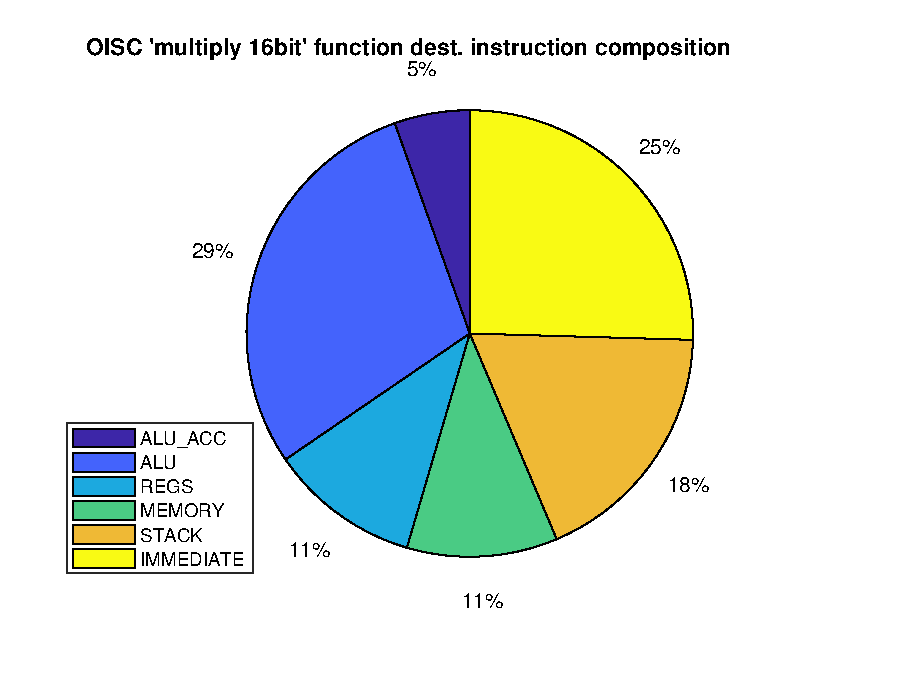
\includegraphics[width=1.3\textwidth]{../tests/oisc_mul16_dst_comp.eps}
		\caption{}
		\label{fig:t2}
	\end{subfigure}
	\caption{Instruction composition experiment results for 16bit multiplication}\label{fig:t}
\end{figure}

Using modelsim, performed simulations on both processors for multiple tasks. Executed instruction have been recorded and further analysed to see function instruction composition.



\pagebreak


\section{Difficulties encountered}
When writing Sieve of Atkins function some unexpected behaviour was encountered. It took quite a bit of time to find 2 causes:
\begin{description}
	\item[$\bullet$] \texttt{ORI} instruction does not behave as it suppose to.
	\item[$\bullet$] 16bit modulus function runs into infinite loop at specific parameters because of \texttt{BGE} (Branch greater than) being used instead of \texttt{BGT} (Branch greater or equal).
\end{description}

Difficulties with tasks management due to COVID-19 chaos.

\section{Failure Risk Assessment}
There are no updates on failure risk assessment. 

\section{Updated Safety Risk Assessment}
There are no updates on safety risk assessment.

\section{Help and Advice Needed}
At this state no help is needed, and any issues and advices are sorted out and discussed in weekly supervisor meetings.

\newpage
\begin{landscape}
	\section{Updated Schedule}
	\begin{table}[h!]
		\centering
		\begin{ganttchart}[
			y unit title=0.4cm,
			y unit chart=0.5cm,
			x unit=1.1mm,
			hgrid,
			today=2020-03-25,
			today label node/.append style={below=12pt},
			today label font=\itshape\color{blue},
			today rule/.style={draw=blue, ultra thick},
			title height=1,
			bar/.append style={fill=blue!50},
			bar incomplete/.append style={fill=gray!50},
			progress label text={$\displaystyle{#1\%}$},
			time slot format=isodate
			]{2019-10-01}{2020-04-14}
			\gantttitlecalendar{year, month=shortname} \\
			\gantttitle{40}{6}
			\gantttitlelist{41,...,52}{7}
			\gantttitlelist{1,...,15}{7}
			\gantttitle{}{2} \\
			\ganttbar[progress=100]{RISC implementation}{2019-10-01}{2019-10-27}\\
			\ganttbar[progress=100]{RISC Optimisations}{2019-10-27}{2019-11-25}\\
			\ganttbar[progress=100]{UART and I/O}{2019-10-21}{2019-10-27}
			\ganttbar[progress=100]{}{2019-11-25}{2019-12-08} \\
			\ganttbar[progress=100]{RISC Assembler}{2019-10-14}{2019-11-11}\\
			\ganttbar[progress=100]{Developing benchmark}{2019-11-11}{2019-12-13}
			\ganttbar[progress=100]{}{2020-02-23}{2020-03-07} \\
			\ganttbar[progress=100]{OISC Implementation}{2019-12-02}{2019-12-13}
			\ganttbar[progress=100]{}{2020-01-13}{2020-02-02}\\
			\ganttbar[progress=100]{OISC Optimisations}{2020-02-02}{2020-02-23}\\
			\ganttbar[progress=100]{OISC Assembler}{2020-01-20}{2020-02-09}\\
			\ganttbar[progress=90]{Benchmarking}{2020-02-17}{2020-03-22}\\
			\ganttmilestone{Project Proposal finalised}{2019-10-14}\\
			\ganttmilestone{Progress Report \#1}{2019-11-04}\\
			\ganttmilestone{Progress Report \#2}{2019-11-25}\\
			\ganttmilestone{December Interim Report}{2019-12-13}\\
			\ganttmilestone{Progress Report \#3}{2020-01-20}\\
			\ganttmilestone{Progress Report \#4}{2020-02-17}\\
			\ganttmilestone{Progress Report \#5}{2020-03-02}\\
			\ganttmilestone{Poster Presentation}{2020-03-18}\\
			\ganttmilestone{Progress Report \#6}{2020-03-24}\\
			\ganttmilestone{Final Report}{2020-04-13}
			\ganttvrule{Reading Week}{2019-11-03}
			\ganttvrule{}{2019-11-10}
			\ganttvrule[vrule label node/.append style={anchor=north west}]{Holidays}{2019-12-13}
			\ganttvrule{}{2020-01-12}
			\ganttvrule{Reading Week}{2020-02-17}
			\ganttvrule{}{2020-02-23}
		\end{ganttchart}	
		\caption{Updated project schedule Grantt chart}
		\label{table:time}
	\end{table}
\end{landscape}

\end{document}